\chapter{Introduction}
\label{ch:intro}

% • In welchem Kontext steht die Aufgabe? -> motivation
% • Was ist der Stand der Technik? -> state of the art
% • Welche L¨ ucke soll die Arbeit schließen? -> objectives
% • Was ist Ihr L¨ osungsansatz? -> approach

Today, 54 percent of the world's population lives in urban
areas.\footnote{\url{https://esa.un.org/unpd/wup/}}
% actually http://www.un.org/en/development/desa/news/population/world-urbanization-prospects-2014.html
In urban areas, public transportation systems are of great importance for its
efficient functioning.
One of the most important types of transportation are suburban trains.
These trains can be almost empty at midday or overcrowded at peak hours.
Depending on the degree of utilization, passengers may have to adapt their
behavior.
If there are free seats available, passengers often choose to sit down for their
journey.
% Fast 1:1 übernommen von Michaels Vorschlag

In this work, I investigate passengers' seating behavior in Munich's suburban
trains and present a simulation model implemented in the crowd simulation
software \vadere.
In the following sections, I outline the motivation and the current state of the
art, and I present the objectives, the approach, and the structure of this work.

\section{Motivation}

Pedestrian dynamics and crowd simulation is a wide field of research
\citep{daamen-2014}.
Crowd simulation can be used to predict evacuation time or crowd density in
evacuation analyses
\citep{kirchner2002simulation,pelechano2006modeling,gao-2014,Alizadeh2011315}.
More generally, such simulations are applicable for the study of places where a
larger number of people come together, \eg in public transport systems and
especially at train stations.
Simulation software can already cope with common scenarios including gates,
queues, stairs, and multiple
floors (\eg \citet{koster-2015,koster-2014b,vadere2016:online}).
Research on people's spatial distribution during waiting times has also brought
useful results (\eg \citet{seitz-2015b,liu-2016,liu-2016b}).
However, there is little research on people's seating behavior, that can be used to
simulate this aspect in the larger system.
% TODO the lack of proper understanding of seating behavior ... leads to ...
There are many questions to be answered, for example ``where do people sit down in
relation to another person?'', ``how do groups of people sit together?'', or
``how does age or gender influence the choice of seating?''.

\section{State of the art}

For literature research I employed the search terms ``choice of seating'' and
``preferred seating'' combined with ``public transport'' and ``trains'' in
English and German.\footnote{I searched in libraries of Munich's major
universities, in Google Scholar, and in Google's standard search
engine. Web of Science and Scopus were not available. The main literature research
was done in February of 2016.}

There is a number of publications on boarding schemes for
airplanes \citep{steiner-2009,jaehn-2015,qiang-2014}.
Some of the studies also provide simulation for the boarding
process \citep{steiner-2009,qiang-2014}.
The goal here is to reduce the boarding time.

Another research focus is on public transportation related to passenger's
behavior in train interiors.
Some studies contain useful hints related to seating behavior, \eg studies on
the degree of capacity utilization \citep{cis-2009}, baggage in
trains \citep{plank-2008}, passenger exchange
times \citep{tuna-2008,panzera-2014}, and train interior
design \citep{rueger-2015}.

Studies on seating layouts and passengers' seating behavior in trains are
discussed by several authors.
\citet{trinkoff-1985} conducted a study on preferred facing directions
in the Washington Metro.
\citet{rueger-2010} surveyed preferred seat choices in inter-city trains.
\citet{wardman-2015} carried out a survey on passengers' valuation of
seating layouts in public transportation.

Other studies are concerned with the inflow process when people enter a
room \citep{liu-2016,liu-2016b,xiao-2016,ezaki-2016}.
While these studies conduct experiments where the subjects cannot sit down, some
aspects are still interesting for this work.
Furthermore, these studies can serve as a starting point for modeling the
behavior of standing passengers in trains, which is not subject of this work.

For pedestrian simulation I mainly build on work done at the \acl{MUAS}, namely
the \vadere\ crowd simulation framework and associated research.
\citet{seitz-2016} presents various research results on pedestrian locomotion
and gives an introduction to \vadere.

% \cite{plank-2008} is about dimensions of Gepackablagen in Reisezügen.
% Passengers want to have a direct sight to their baggage. See notes.

% \cite{tuna-2008} is about Fahrgastwechselzeit im Personenfernverkehr. Evtl. auch
% Datenerhebungen in Nahverkehrszügen? See notes.

% \cite{panzera-2014} Haltezeiten bei Personennahverkehr: Einflussfaktoren!

% \cite{rueger-2015} Innenraum von Reisezügen (über effiziente Gestaltung).

% \cite{cis-2009} Auslastungsgrad von Eisenbahnwagen in Abhängigkeit von
% individuellem Fahrgastverhalten.

\section{Objectives}

Although there is a number of studies on seating behavior in public
transportation, there is no detailed data available for a deeper analysis of
various aspects of the choice of seating.
To my knowledge, there are also no models or algorithms available to simulate
the inflow and the seating process in trains.
In this work, I therefore investigate passengers' seating behavior in trains
from an empirical point of view and develop a simulation model for the crowd
simulation software \vadere.

The objectives are two-fold.
First, I want to promote simulations of public transportation systems by
adding one part to the collection of simulation models: A model to simulate
seating behavior.
Second, I want to set up a framework for data collection and provide data from
my study for social psychology research.
This has a great potential for synergy because findings used for the model can
also be interesting for the study of social behavior of individuals or groups
in psychology.

\section{Approach}

In this work, I apply empirical and formal methods:
I collect data in a field observation, and I develop an algorithmic model that
describes seating behavior of passengers in trains.

First, I conduct the data collection in Munich's \sbahn\ to explore passengers'
seating behavior within compartments.
The data collection is an observational field study in which events in the train
are logged in real-time.
How passengers spread through the train wagon is not covered by the study.

Second, I develop a theoretical model for seating behavior based on the
collected data using a combination of cognitive heuristics and statistics.
and, I implement the model in the crowd simulation software \vadere\ and
verify it against the collected data.

\section{Structure of this work}

In chapter~\ref{ch:data}, Data collection, I gather requirements for the
data collection and for a software tool to conduct the data collection.
I present the resulting app's \acs{UI} and usage.
After a pilot study the main study on seating behavior is conducted and the
procedure of data processing is explained.
I describe data on passenger counts which was made available from the
\acf{MVV}, and I collected and analyzed passenger entrance rates.

In chapter~\ref{ch:software}, Software, I describe some aspect of the data
collection app's architecture, design, and development.
I introduce the crowd simulation software \vadere\ and state contributions to
\vadere, which are required for a good integration of the seating model.
I present the \traingen\ tool for generating train scenarios which can be
imported in \vadere.
Finally, the seating model's software design and implementation are described
together with the system for model validation.

In chapter~\ref{ch:model}, Model, I first specify approach, assumptions, and
limitations of the seating model.
I analyze the collected data on seating behavior and develop a model based on
these results.
Then, I explain the model's algorithms and parameters in detail.

In chapter~\ref{ch:evaluation}, Model~evaluation, I first verify the model's
implementation by comparing simulated data against real data.
Second, I visually validate the model by demonstrating that the train fills up
in a realistic manner.
Both methods are based on a simulation run with real passenger counts.

The conclusions give a short summary of the results, discussions, and
inspiration for future work in this field.

\section{Terms and definitions}
\label{sec:terms}

In the following, I define terms used to describe the train interior.

\begin{description}

  \item[Entrance area] The room between two opposing doors.

  \item[Compartment] The room between two adjacent entrance areas.
    There are 16 seats per compartment.

  \item[Seat group] A group of four vis-a-vis seats, that is two facing benches.

  \item[Seat number] Seats are numbered within a compartment, row by row.
    A row is four seats facing the same direction.
    The numbers range from 1 to 16 and increase from left to right and
    from the front to the rear.
    Front and rear can be defined arbitrarily but the seat numbering must not
    change when the train changes its driving direction.
    Figure~\ref{fig:compartment} illustrates the seat numbering schema.
    The numbering schema is also implemented in the app for data collection as
    depicted in figure~\ref{fig:app-screen-3}.

  \item[Compartment plan] A top view plan of the compartment including a
    correct seat numbering \eg figure~\ref{fig:compartment} is such a plan.

\end{description}

\begin{figure}[htb]
  \centering
  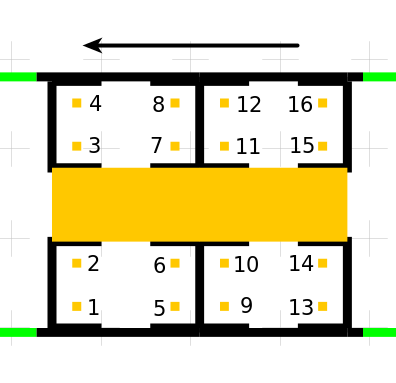
\includegraphics[width=8cm]{compartment}
  \caption[Plan of a \sbahn\ train compartment.]{%
    This figure shows a plan of a \sbahn\ train compartment with four seat
    groups, each consisting of four seats.
    The black arrow on the top denotes the train's driving direction.
    The yellow dots mark the seats and the yellow area in the middle is the
    aisle connecting the entrance areas.
    The green bars are parts of the doors.
  }\label{fig:compartment}
\end{figure}

\section{Conventions}

\subsection{Reproducible research}

I strive to do reproducible research in this thesis
\citep{peng2011reproducible}.
To achieve this goal, I use the following techniques:

\begin{itemize}[noitemsep,nolistsep]

  \item All plots are generated with knitr \citep{knitr2:online} at the moment
    this \LaTeX~document is compiled.

  \item All numbers are either generated with knitr or have a footnote like
    this\footnote{\verb~echo -n "this"~\shellcmdline}, to provide the shell code
    to reproduce the value.

  \item Sample data, tables, and sample output of programs are taken from their
    sources or generated in the process of compiling this document.

  \item Code samples and listings are taken from their original source files.
    This is made possible with \code{Makefile}s, shell scripts, and the
    \verb|\lstinputlisting| command from the
    \href{https://www.ctan.org/pkg/listings}{Listings} package.

  \item Listings that show interfaces of Java classes are generated with the
    \code{javap} program\footnote{The \code{javap} tool is distributed with
    Java; see \verb|javap --help| for more information.}, which can disassemble
    a compiled Java program and extract the interface of a class.

\end{itemize}

To reproduce and verify this work, the \LaTeX~code and the \code{Makefile} can be
examined, R code for plots and statistics can be re-evaluated, and shell command
lines in footnotes can be interpreted.

\subsection{Formatting}

\begin{description}

  \item[\emph{Italic}] font is used when describing user interfaces.
    It is used for labels of \acs{UI} elements such as buttons or menu items.
    It is also used in the text for file or folder names.

  \item[\code{Constant width}] font is used for in-line code snippets and identifiers
    such as function or class names.

\end{description}
